\documentclass[12pt,a4paper]{article}

% Paquetes básicos
\usepackage[utf8]{inputenc}
\usepackage[T1]{fontenc}
\usepackage[english]{babel}
\usepackage{amsmath, amssymb}
\usepackage{siunitx} 
\usepackage{graphicx}
\usepackage{float}
\usepackage{geometry}
\usepackage{xcolor}
\geometry{margin=2.5cm}
\usepackage{hyperref}
\usepackage{caption}
\usepackage{subcaption}
\usepackage{setspace}
\usepackage{multirow}
\usepackage{minted}  
\usepackage{gensymb} 
\usepackage[backend=biber, style=ieee]{biblatex}
\usepackage{csquotes}
\usepackage{indentfirst}
\addbibresource{references.bib}

\graphicspath{{Figures/}}
\onehalfspacing
\hypersetup{
    colorlinks  = true,
    linkcolor   = blue,    
    citecolor   = blue,
    urlcolor    = blue,
    filecolor   = blue
}

\begin{document}       
\renewcommand{\figureautorefname}{Fig.}
\renewcommand{\tableautorefname}{Tab.}
\renewcommand{\equationautorefname}{Eq.}


% Carátula personalizada
\begin{titlepage}
    \centering
    
\includegraphics[width=0.7\textwidth]{Fulgor Logo.png}\\[1.5cm]

    {\Large \textbf{FUNDACIÓN FULGOR} \\[0.5cm]}
    {\Large CMOS Course} \\[0.5cm]

    \rule{\textwidth}{0.5pt} \\[0.5cm]
    {\Large \textbf{Homework N°1} \\[0.3cm]}
    \rule{\textwidth}{0.5pt} \\[1cm]
    
\begin{tabular}{l l}
    \textbf{Profesores:} & Michel Saenz.\\
                         & Santiago Castro.\\
    \\
    \textbf{Alumno:} & Monja, Ernesto Joaquín (43.873.728)\\
\end{tabular} \\[5cm]

{\centering Año 2026 \par}

\end{titlepage}



% Índice
\tableofcontents
\newpage



\section{Introduction}
This document presents the solutions for Homework $\#01$ of the \textit{CMOS} Course of Fulgor Foundation. The primary objective of this assignment is to review and consolidate fundamental concepts in analog  \textit{CMOS} transistor behavior.

The report is divided into three main sections:
\begin{itemize}
    \item A theoretical analysis of the Current-Voltage ($I/V$) characteristics of  \textit{PMOS} devices, highlighting the terminal definitions and equation differences relative to \textit{NMOS} transistors.
    \item A comprehensive summary of critical second-order effects in \textit{MOS} transistors, detailing the physical phenomena, their electrical impact, and their corresponding mathematical models.
    \item A practical \textit{DC} analysis of several basic circuit topologies to systematically determine the region of operation for individual MOS transistors.
\end{itemize}



\section{PMOS Transistor I/V Characteristics}
In a \textit{PMOS} transistor, the charge carriers are holes and the terminal voltages $V_{GS}$, $V_{DS}$, as well as the threshold voltage $V_{TH}$, are inherently negative numbers during normal operation. Following the convention adopted in Razavi's \textit{Fundamentals of Microelectronics}, we employ absolute values ($|V_{GS}|$, $|V_{DS}|$, and $|V_{TH}|$) to define the regional boundaries and current equations using positive parameters.

In \autoref{fig:fig_1} we can see the Structure of \textit{PMOS} device (a), the \textit{PMOS} circuit symbol (b) and an illustration of triode and saturation regions based on gate and drain voltages (c).
\begin{figure}[H]
    \centering
    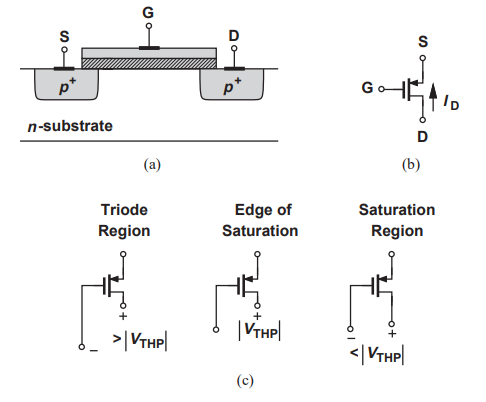
\includegraphics[width=0.5\linewidth]{Figure 1.png}
    \caption{Structure, Circuit Symbol and Regions of a PMOS transistor. \cite[p. 296]{b1}} 
    \label{fig:fig_1}
\end{figure}

The regions of operation are classified as follows:
\begin{itemize} 
    \item \underline{Triode Region:} Also known as the \textit{Linear Region}, this is when the conducting channel is formed and the device acts as a voltage-controlled resistor. This occurs under the following conditions:
    \begin{equation}
        |V_{GS}| > |V_{TH}| \quad \text{and} \quad |V_{DS}| < |V_{GS}| - |V_{TH}|
        \label{eq_1}
    \end{equation}
    The resulting drain current $I_{D}$ is expressed as:
    \begin{equation}
        I_{D,tri} = -\frac{1}{2} \mu_p C_{ox} \frac{W}{L} \left[2 (V_{GS} - V_{TH})V_{DS} - V_{DS}^{2} \right]
        \label{eq_2}
    \end{equation}
    
    \item \underline{Saturation Region:} The channel pinches off near the drain terminal, meaning the current becomes heavily independent of $V_{DS}$. This condition is met when:
    \begin{equation}
        |V_{GS}| > |V_{TH}| \quad \text{and} \quad |V_{DS}| \ge |V_{GS}| - |V_{TH}|
        \label{eq_3}
    \end{equation}
    Neglecting channel-length modulation, the saturation drain current is given by:
    \begin{equation}
        I_{D,sat} = -\frac{1}{2} \mu_p C_{ox} \frac{W}{L} (V_{GS} - V_{TH})^{2} ( 1- \lambda V_{DS})
        \label{eq_4}
    \end{equation}
    where $\lambda$ represents the channel-length modulation parameter.

    \item \underline{Cutoff Region:} The transistor remains turned off when the absolute gate-to-source voltage is insufficient to invert the channel, this is:
    \begin{equation}
        |V_{GS}| < |V_{TH}| \implies I_{D,cut} = 0
        \label{eq_5}
    \end{equation}
\end{itemize}

In \autoref{fig:fig_2}, we can notice that given the notation of $V_{DS}$ rather than $V_{SD}$ and the negative sign in \autoref{eq_2} and \autoref{eq_4}, its expected that the regions are to be found in the third quadrant.
\begin{figure}[H]
    \centering
    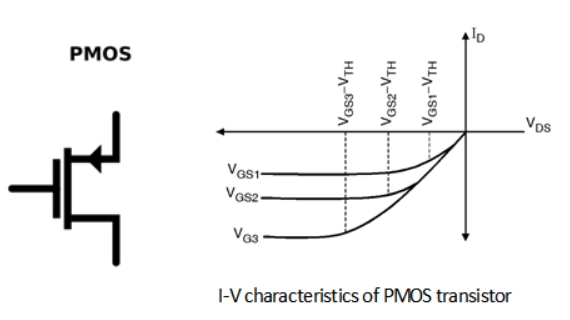
\includegraphics[width=0.6\linewidth]{Figure 2.png}
    \caption{I/V Characteristics of a \textit{PMOS} transistor. \cite{b2}} 
    \label{fig:fig_2}
\end{figure}



\section{Summary of 2nd Order Effects in \textit{MOS} Transistors}
\subsection{Channel-Length Modulation}
\begin{itemize}
    \item \underline{Physical Phenomenon:} In the saturation region, as $V_{DS}$ increases beyond the overdrive voltage ($V_{GS} - V_{TH}$), the depletion region surrounding the drain expands. This causes the channel pinch-off point to move slightly away from the drain towards the source, effectively reducing the electrical channel length ($L_{eff} = L - \Delta L$). 
    \item \underline{Electrical Impact:} The drain current $I_{D}$ preserves a slight linear dependence on $V_{DS}$ even within the saturation region. This gives rise to a finite output resistance ($r_o$) rather than an ideal infinite value.
    \item \underline{Mathematical Representation:} The mathematical representation of the Channel-Length Modulation can be seen in \autoref{eq_4}.
\end{itemize}


\subsection{Body Effect}
\begin{itemize}
    \item \underline{Physical Phenomenon:} When the bulk (substrate) is biased at a different potential than the source ($V_{SB} > 0$), the resulting reverse-bias voltage widens the depletion layer beneath the gate oxide. This exposes additional immobile ions in the substrate.
    \item \underline{Electrical Impact:} More gate voltage is required to establish the inversion layer and open the channel. Consequently, the threshold voltage ($V_{TH}$) increases as $V_{SB}$ increases.
    \item \underline{Mathematical Representation:} This phenomenon can be expressed according to the \autoref{eq_6}.
    \begin{equation}
        V_{TH} = V_{TH0} + \gamma \left( \sqrt{|2\Phi_F + V_{SB}|} - \sqrt{|2\Phi_F|} \right)
        \label{eq_6}
    \end{equation}
    where $V_{TH0}$ is the nominal threshold voltage for $V_{SB}=0$, $\gamma$ is the body-effect coefficient, and $\Phi_F$ is the Fermi potential of the substrate, where these last two variables are technology-dependent parameters having typical values of $0.4\sqrt{V}$ and $0.4 V$, respectively. \cite[p. 293]{b1}
\end{itemize}


\subsection{Subthreshold Conduction}
\begin{itemize}
    \item \underline{Physical Phenomenon:} When $V_{GS}$ drops below $V_{TH}$, the channel charge does not abruptly drop to zero. Instead, a weak inversion layer remains at the silicon surface, allowing current to flow primarily via carrier diffusion instead of drift.
    \item \underline{Electrical Impact:} The transistor exhibits an exponential leakage current with respect to $V_{GS}$. This behavior is a dominant factor in off-state power consumption and low-power circuit topologies.
    \item \underline{Mathematical Representation:} This phenomenon can be expressed according to the \autoref{eq_7}.
    \begin{equation}
        I_{D} = I_{0} e^{\left( \frac{V_{GS} - V_{TH}}{n V_T} \right)}
        \label{eq_7}
    \end{equation}
    where $n$ represents the subthreshold slope factor, $V_T = kT/q$ is the thermal voltage, and $I_0$ is a baseline current constant.
\end{itemize}



\section{Region of Operation of \textit{M1}}
To determine the operating region of the MOS transistors in the provided circuits, we must analyze the node voltages ($V_G$, $V_D$, $V_S$) to find $V_{GS}$ and $V_{DS}$. Assuming a generic threshold voltage $V_{th}$ for the NMOS devices, we apply the following conditions:
\begin{enumerate}   
    \item \textbf{Triode (Linear):} If $V_{GS} > V_{th}$ and $V_{DS} < V_{GS} - V_{th}$, the transistor is in the triode region.
    \item \textbf{Saturation:} If $V_{GS} > V_{th}$ and $V_{DS} \ge V_{GS} - V_{th}$, the transistor is in saturation. (Also holds true if the drain is tied to the gate, $V_{DS} = V_{GS}$, ensuring $V_{DS} > V_{GS} - V_{th}$).
    \item \textbf{Cutoff:} If $V_{GS} < V_{th}$, the transistor is OFF.
\end{enumerate}

The circuits that will be analyzed are shown in \autoref{fig:fig_3} divided in two sub-figures named \textit{Figure 6.38} and \textit{Figure 6.39}.
\begin{figure}[H]
    \centering
    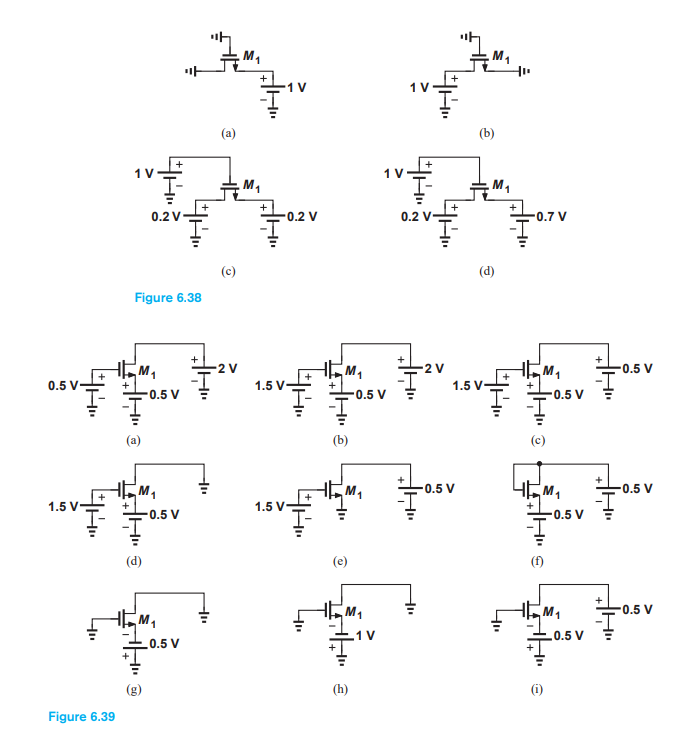
\includegraphics[width=0.6\linewidth]{Figure 3.png}
    \caption{Circuits to be analyzed. \cite[p. 302]{b2}} 
    \label{fig:fig_3}
\end{figure}

In \autoref{tab:tab_1}, it is shown for each circuit in \autoref{fig:fig_3}, the values of each terminal of the \textit{NMOS} transistor and in which region it operates.
\begin{table}[H]
    \centering
    \renewcommand{\arraystretch}{1.4}
    \begin{tabular}{|c|c|c|} \hline
        \textbf{Circuit} & \textbf{Node Voltages} & \textbf{Region of Operation} \\ \hline
        Fig. 6.38 ; Circ. (a) & $V_{G} = 0 \ [V]$, $V_{S} = 0 \ [V]$, $V_{D} = 1 \ [V]$ & Cutoff \\ \hline
        Fig. 6.38 ; Circ. (b) & $V_{G} = 0 \ [V]$, $V_{S} = 1 \ [V]$, $V_{D} = 0 \ [V]$ & Cutoff \\ \hline
        Fig. 6.38 ; Circ. (c) & $V_{G} = 1 \ [V]$, $V_{S} = 0.2 \ [V]$, $V_{D} = 0.2 \ [V]$ & Triode \\ \hline
        Fig. 6.38 ; Circ. (d) & $V_{G} = 1 \ [V]$, $V_{S} = 0.2 \ [V]$, $V_{D} = 0.7 \ [V]$ & Saturation \\ \hline
        Fig. 6.39 ; Circ. (a) & $V_{G} = 0.5 \ [V]$, $V_{S} = 0.5 \ [V]$, $V_{D} = 2 \ [V]$ & Cutoff \\ \hline
        Fig. 6.39 ; Circ. (b) & $V_{G} = 1.5 \ [V]$, $V_{S} = 0.5 \ [V]$, $V_{D} = 2 \ [V]$ & Saturation \\ \hline
        Fig. 6.39 ; Circ. (c) & $V_{G} = 1.5 \ [V]$, $V_{S} = 0.5 \ [V]$, $V_{D} = 0.5 \ [V]$ & Triode \\ \hline
        Fig. 6.39 ; Circ. (d) & $V_{G} = 1.5 \ [V]$, $V_{S} = 0.5 \ [V]$, $V_{D} = 0 \ [V]$ & Triode \\ \hline
        Fig. 6.39 ; Circ. (e) & $V_{G} = 1.5 \ [V]$, $V_{S} = 0 \ [V]$, $V_{D} = 0.5 \ [V]$ & Triode \\ \hline
        Fig. 6.39 ; Circ. (f) & $V_{G} = 0.5 \ [V]$, $V_{S} = 0.5 \ [V]$, $V_{D} = 0.5 \ [V]$ & Cutoff \\ \hline
        Fig. 6.39 ; Circ. (g) & $V_{G} = 0 \ [V]$, $V_{S} = -0.5 \ [V]$, $V_{D} = 0 \ [V]$ & Saturation \\ \hline
        Fig. 6.39 ; Circ. (h) & $V_{G} = 0 \ [V]$, $V_{S} = -1 \ [V]$, $V_{D} = 0 \ [V]$ & Saturation \\ \hline
        Fig. 6.39 ; Circ. (i) & $V_{G} = 0 \ [V]$, $V_{S} = -0.5 \ [V]$, $V_{D} = 0.5 \ [V]$ & Saturation \\ \hline
    \end{tabular}
    \caption{Summary of operating regions for transistors in Figures 6.38 and 6.39. A threshold voltage of $|V_{TH}| = 0.4 \ [V]$ is assumed for all \textit{NMOS} transistors.}
    \label{tab:tab_1}
\end{table}


\section{Conclusion}
This assignment successfully reinforced the foundational principles of analog \textit{CMOS} behavior, bridging theoretical device physics with practical circuit analysis. By examining the \textit{PMOS} transistor through \textit{Razavi}'s absolute-value convention, a unified and mathematically robust approach to defining regions of operation was established. 

Furthermore, the exploration of second-order effects, such as \textit{Channel-Length Modulation}, the \textit{Body Effect}, and \textit{Subthreshold Conduction}, highlighted the critical deviations from ideal models that must be accounted for in modern deep-submicron \textit{IC} design.

Finally, the systematic \textit{DC} analysis of various basic \textit{MOS} topologies consolidated the ability to accurately determine node potentials and operating regions. Mastering these fundamental concepts is an essential stepping stone for the subsequent design and analysis of more complex analog integrated circuits.



\newpage
\printbibliography[heading=bibintoc, title={6 \ Bibliography}]

\end{document}